\documentclass[aspectratio=43,10pt]{beamer}

\usetheme[progressbar=frametitle]{metropolis}
\usepackage{appendixnumberbeamer}
\usepackage{booktabs}
% \usepackage[scale=2]{ccicons}
\usepackage{pgfplots}
\usepgfplotslibrary{dateplot}
\usepackage{xspace}
\usepackage[english,main=brazilian]{babel}
\usepackage[utf8x]{inputenc}
\usepackage[alf]{abntex2cite}
\usepackage{multirow}
\usepackage{ragged2e}
\usepackage{xspace}

\usepackage{pgfgantt}
\usepackage[inline]{enumitem}

\title[]{Uma Implementação Distribuída em Névoa do Algoritmo de Detecção de
Novidade em Fluxos de Dados MINAS}
% \subtitle{Seminários de Metodologia Científica}
\author{Luís Henrique Puhl de Souza\\
Orientador: Prof. Dr. Hermes Senger}
\institute{
Universidade Federal de São Carlos \\
Centro de Ciências Exatas e de Tecnologia \\
Departamento de Computação \\
Programa de Pós-Graduação em Ciência da Computação}
% \date{\today}
\date{Fevereiro 2020}
% \titlegraphic{\hfill\includegraphics[height=1.5cm]{logo.pdf}}

\newcommand{\nota}[1]{\hspace*{-0.5cm}\textit{{\color[rgb]{1,0,0}Nota: #1}}}

\begin{document}

\maketitle

\begin{frame}{Índice}
  \setbeamertemplate{section in toc}[sections numbered]
  \tableofcontents[hideallsubsections]
\end{frame}

\section{Introdução}

\begin{frame} [fragile]{Introdução}
\begin{itemize}

% Contexto Geral
\item Crescimento do número de dispositivos IoT e riscos associados;

% Contexto Específico
\item Detecção de intrusão em redes por novidade

% Proposta
\item Um sistema para detecção de intrusão em Redes IoT implementando em névoa

% hipótese
\item A hipótese do trabalho é que o algoritmo MINAS pode ser distribuído em
nós de nuvem e névoa reduzindo a latência e com pouco comprometimento na
qualidade de detecção.

\end{itemize}

\nota{pode falar:\\
- dificuldade de atualização de SW\\
- como foi o ataque MIRAI? (só curiosidade)\\
- capacidade de autodefesa? mesmo outros computadores não têm...}
\end{frame}


\section{Fundamentos}
\begin{frame}[fragile]{Fundamentos}
\begin{itemize}
\item Ambientes de computação Distribuída;
\item Plataformas de processamento distribuído de fluxos;
\item Métodos Detecção de Novidade;
\end{itemize}
\nota{Por que "seria dificil processar de forma centralizado"?}
\end{frame}

\begin{frame}[fragile]{Fundamentos}

\metroset{block=fill}

\begin{block}{Definição de Fluxo de Dados}
  
  \vspace{5mm}
  Defu

  \begin{itemize}
    \item Evolução;
    \item Mudança;
    \item Ruído;
  \end{itemize}
\end{block}
\end{frame}

\newcommand{\novelty}{\emph{Novelty Detection}\xspace}
\newcommand{\nd}{ND\xspace}
\newcommand{\drift}{\emph{Concept Drift}\xspace}
\newcommand{\evolution}{\emph{Concept Evolution}\xspace}

\begin{frame}[fragile]{Fundamentos}
  \begin{alertblock}{Métodos Detecção de Novidade}
    
    \vspace{5mm}
    Métodos Detecção de Novidade (\novelty) lidam com o reconhecimento e
    classificação de exemplos em padrões que diferem de padrões anteriores
    \cite{PERNER2007,Gama2010}.
  
    Conforme \citeonline{Gama2010}, são características de fluxos de dados contínuos:
    \begin{itemize}
      \item Evolução de conceito (\evolution);
      \item Mudança de conceito (\drift, deriva ou desvio);
      \item Ruído e \emph{outliers};
    \end{itemize}
  \end{alertblock}
\nota{Poderia explicar melhor a evolução de modelos, "concept drift"
(precisa estudar um pouco + a teoria).}
\end{frame}

\begin{frame}[fragile]{Fundamentos}
\begin{alertblock}{Ambientes de computação Distribuída}
\begin{itemize}
  \item Computação em Nuvem (\emph{Cloud Computing}):
  \\ \textbf{Características:}
  Serviço sob Demanda,
  Amplo acesso à rede,
  Agrupamento de recursos,
  Elasticidade,
  Serviço mensurado;
  \\ \textbf{Implementações:}
    Nuvem privada,
    Nuvem comunitária,
    Nuvem pública,
    Nuvem híbrida
    \cite{NIST2011}.
  
\end{itemize}
\end{alertblock}
\nota{Separar os items em bullets (sub-bullets)}
\end{frame}

{%
\setbeamertemplate{frame footer}{Terminologia continua incerta entre \emph{fog} e \emph{edge}.}
\begin{frame}[fragile]{Fundamentos}
  \begin{alertblock}{Ambientes de computação Distribuída}
  \begin{itemize}
    
  \item Computação de Borda (\emph{Edge Computing}) \cite{Shi2016}:
  \\ Refere-se a qualquer recurso computacional ou de rede entre os dispositivos
  de borda e centro de dados hospedados em nuvem.
  
  \item Computação em Névoa (\emph{Fog Computing}) \cite{Bonomi2012,dastjerdi2016}:
  \\ \textbf{Características:}
  Mobilidade,
  Heterogeneidade,
  Baixa Latência,
  Distribuição geográfica,
  Alto número de nós,
  Interoperabilidade e federação,
  Uso de fluxo de dados e aplicações em tempo real
  \cite{IEEECommunicationsSociety2018}.
\end{itemize}
\end{alertblock}
\nota{Definição de Fog e borda...\\
São intercambeáveis mesmo?\\
(*Evite colocar questões inconclusivas)}
\end{frame}
}


\begin{frame}[fragile]{Fundamentos}
\begin{alertblock}{Plataformas de processamento distribuído de fluxos}
  \begin{itemize}
    \item Mineração de Dados e Fluxo de Dados;
    \item Arquiteturas \emph{Lambda} e \emph{Kappa};
    \item \emph{MapReduce} e \emph{Apache Hadoop};
    \item \emph{Apache Spark}, \emph{Resilient Distributed Dataset} e
    \emph{micro-batching} para \emph{Spark Streaming};
    \item \emph{Apache Storm};
    \item \emph{Apache Flink};
  \end{itemize}
\end{alertblock}
\nota{Faltou definir antes o que é processamento de fluxo.\\
\textbf{fluxo vs lote} deixar mais claro a diferença}

\nota{O slide fala de plataformas, mas vc falou de kappa e lambda
que não deveria falar neste slide}

\nota{Muita fala p/ esse slide (ficou explicando cada fundamento).
Deveria quebrar o slide em 3 ou 4 slides ao menos.}
\end{frame}

\begin{frame}[fragile]{Fundamentos}
\begin{figure}[ht]
\centering
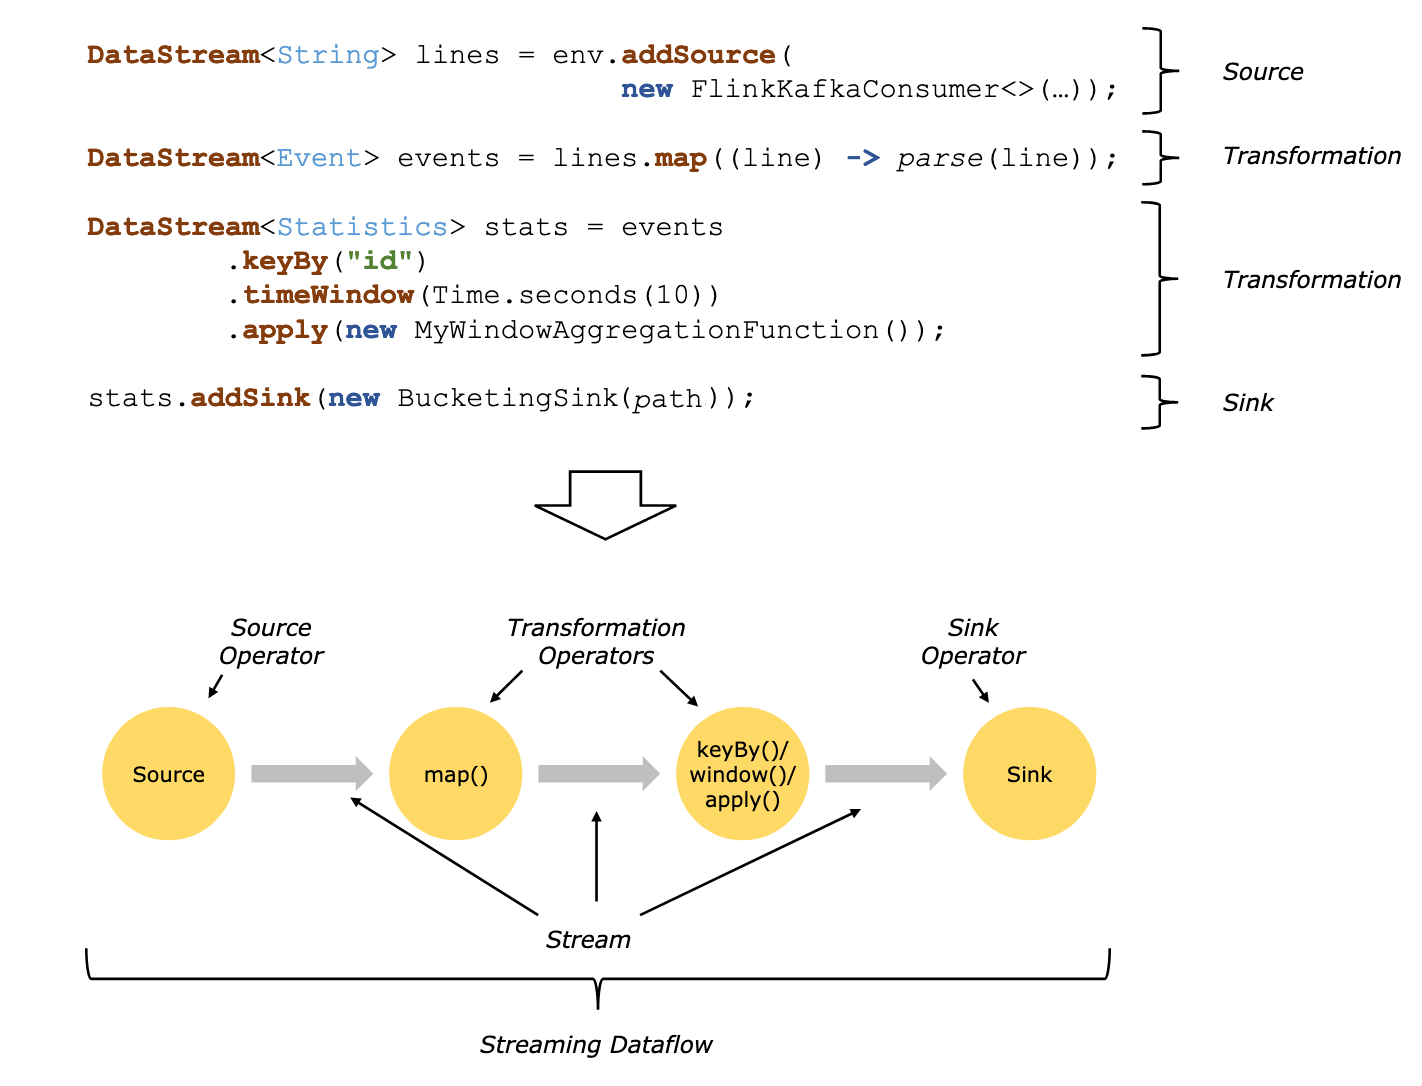
\includegraphics[width=0.85\textwidth]{figuras/dataflow-code-flink.png}
\caption{Exemplo de código e \emph{data flow} do \emph{Apache Flink} \cite{ApacheFlink2020}}
\label{fig:dataflow-flink}
\end{figure}
\end{frame}

\begin{frame}[fragile]{Fundamentos}
\begin{alertblock}{Algoritmo MINAS}
  \vspace{5mm}
  Algoritmo e suas estratégias:
  \begin{itemize}
    \item Modelo de aprendizado \emph{Offline-Online};
    \item Transformação dos dados analisados para o espaço $\mathbb{R}^d$;
    \item Função de classificação baseada em distância euclideana;
    \item Modelo de classificação com \emph{Clusters};
    \item Algoritmo de agrupamento para identificação de padrões;
  \end{itemize}
\end{alertblock}
\nota{MINAS: Use figura!\\pseudocodigo?}
\end{frame}

\begin{frame}[fragile]{Fundamentos}
\begin{figure}[ht]
\centering
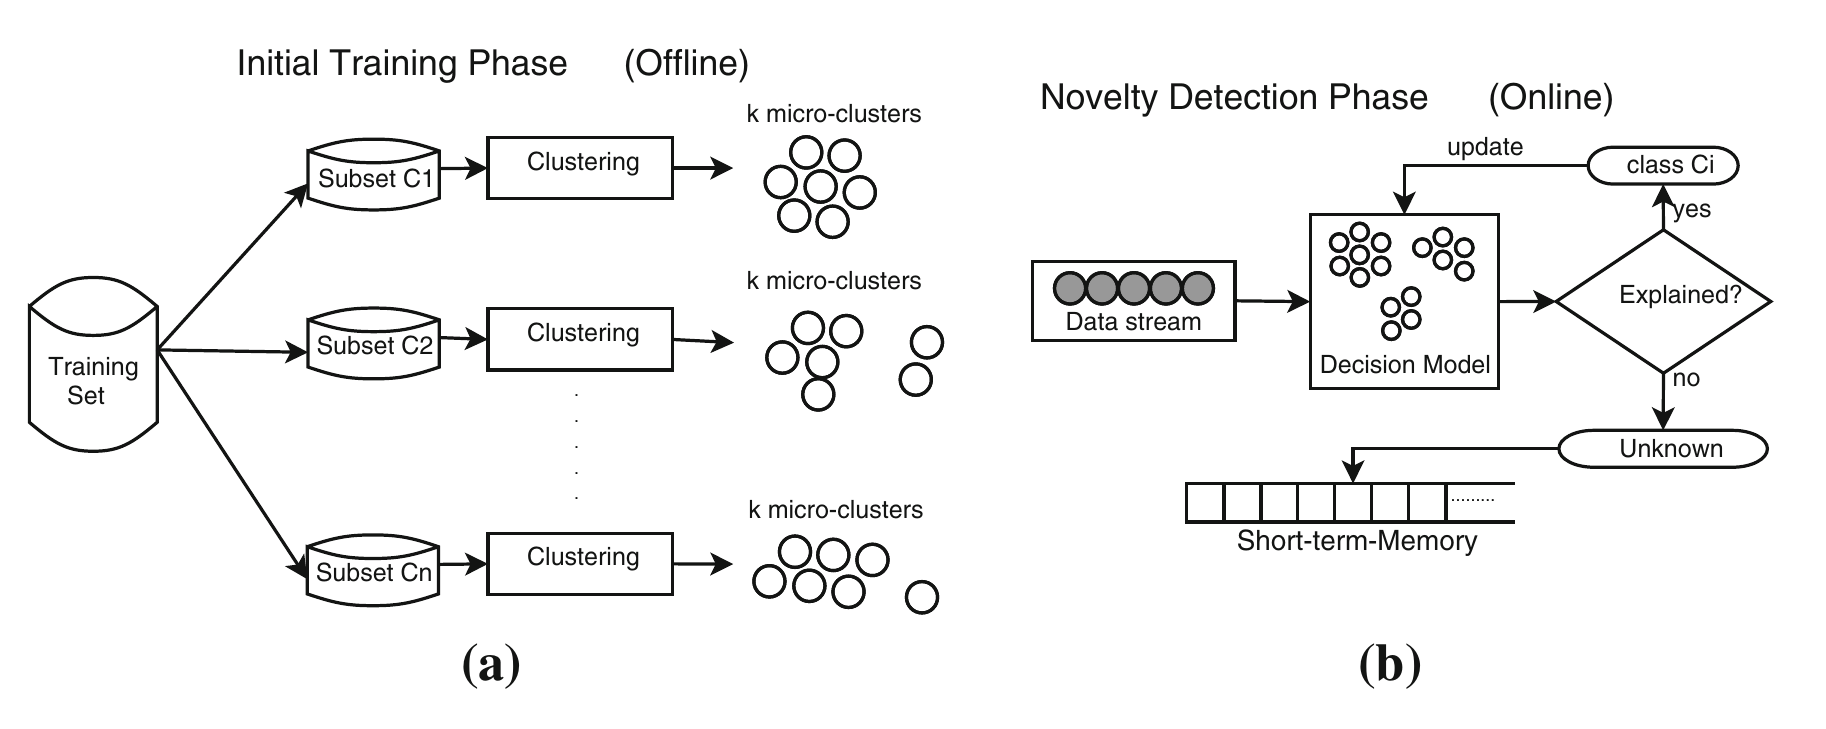
\includegraphics[width=\textwidth]{figuras/FariaMinas2015-fases.png}
\caption{Visão geral do algoritmo MINAS com fases \emph{Offline} (a) e 
\emph{Online} (b) \cite{Faria2016minas}}
\label{fig:minas}
\end{figure}
\nota{Explique o desenho! o que significa cada objeto da figura? explique na figura.}
\end{frame}


\section{Estado da Arte e Trabalhos Relacionados}
\begin{frame}[fragile]{Estado da Arte e Trabalhos Relacionados}
\begin{itemize}
\item Extensões do Algoritmo MINAS;
\item Sistemas de detecção de intrusão em redes;
\end{itemize}
\nota{Trabalhos relacionados * extensões? esses são seus concorrentes?\\
qual é a relação?\\
MEIO FORA DE FOCO!}
\end{frame}

\begin{frame}[fragile]{Estado da Arte e Trabalhos Relacionados}
\begin{alertblock}{Extensões do Algoritmo MINAS}
  \begin{itemize}
    \item FuzzyND: extensão do algoritmo original para classificação com
    conjunto de etiquetas \emph{fuzzy} \cite{DaSilva2018,DaSilva2018thesis};
    \item MINAS-LC e MINAS-BR: extensão do algoritmo original tratando
    classificação multi-etiquetas \cite{Costa2019,Costa2019thesis};
  \end{itemize}
\end{alertblock}
\end{frame}

\newcommand{\idsiot}{IDSA-IoT\xspace}

\begin{frame}[fragile]{Estado da Arte e Trabalhos Relacionados}
\begin{alertblock}{Sistemas de detecção de intrusão em redes}
  \begin{itemize}
    \item Ferramenta BigFlow \cite{Viegas2019};
    \item Ferramenta CATRACA \cite{Lopez2018};
    \item Arquitetura \idsiot \cite{Cassales2019a};
  \end{itemize}
\end{alertblock}
\nota{OK, isso é trabalho relacionado!\\
Dissecar melhor [bigflow, catraca, idsa-iot]\\
passar mais rápido, detalhar nos próximos.}
\end{frame}

\begin{frame}[fragile]{Estado da Arte e Trabalhos Relacionados}
\begin{figure}[ht]
  \centering
  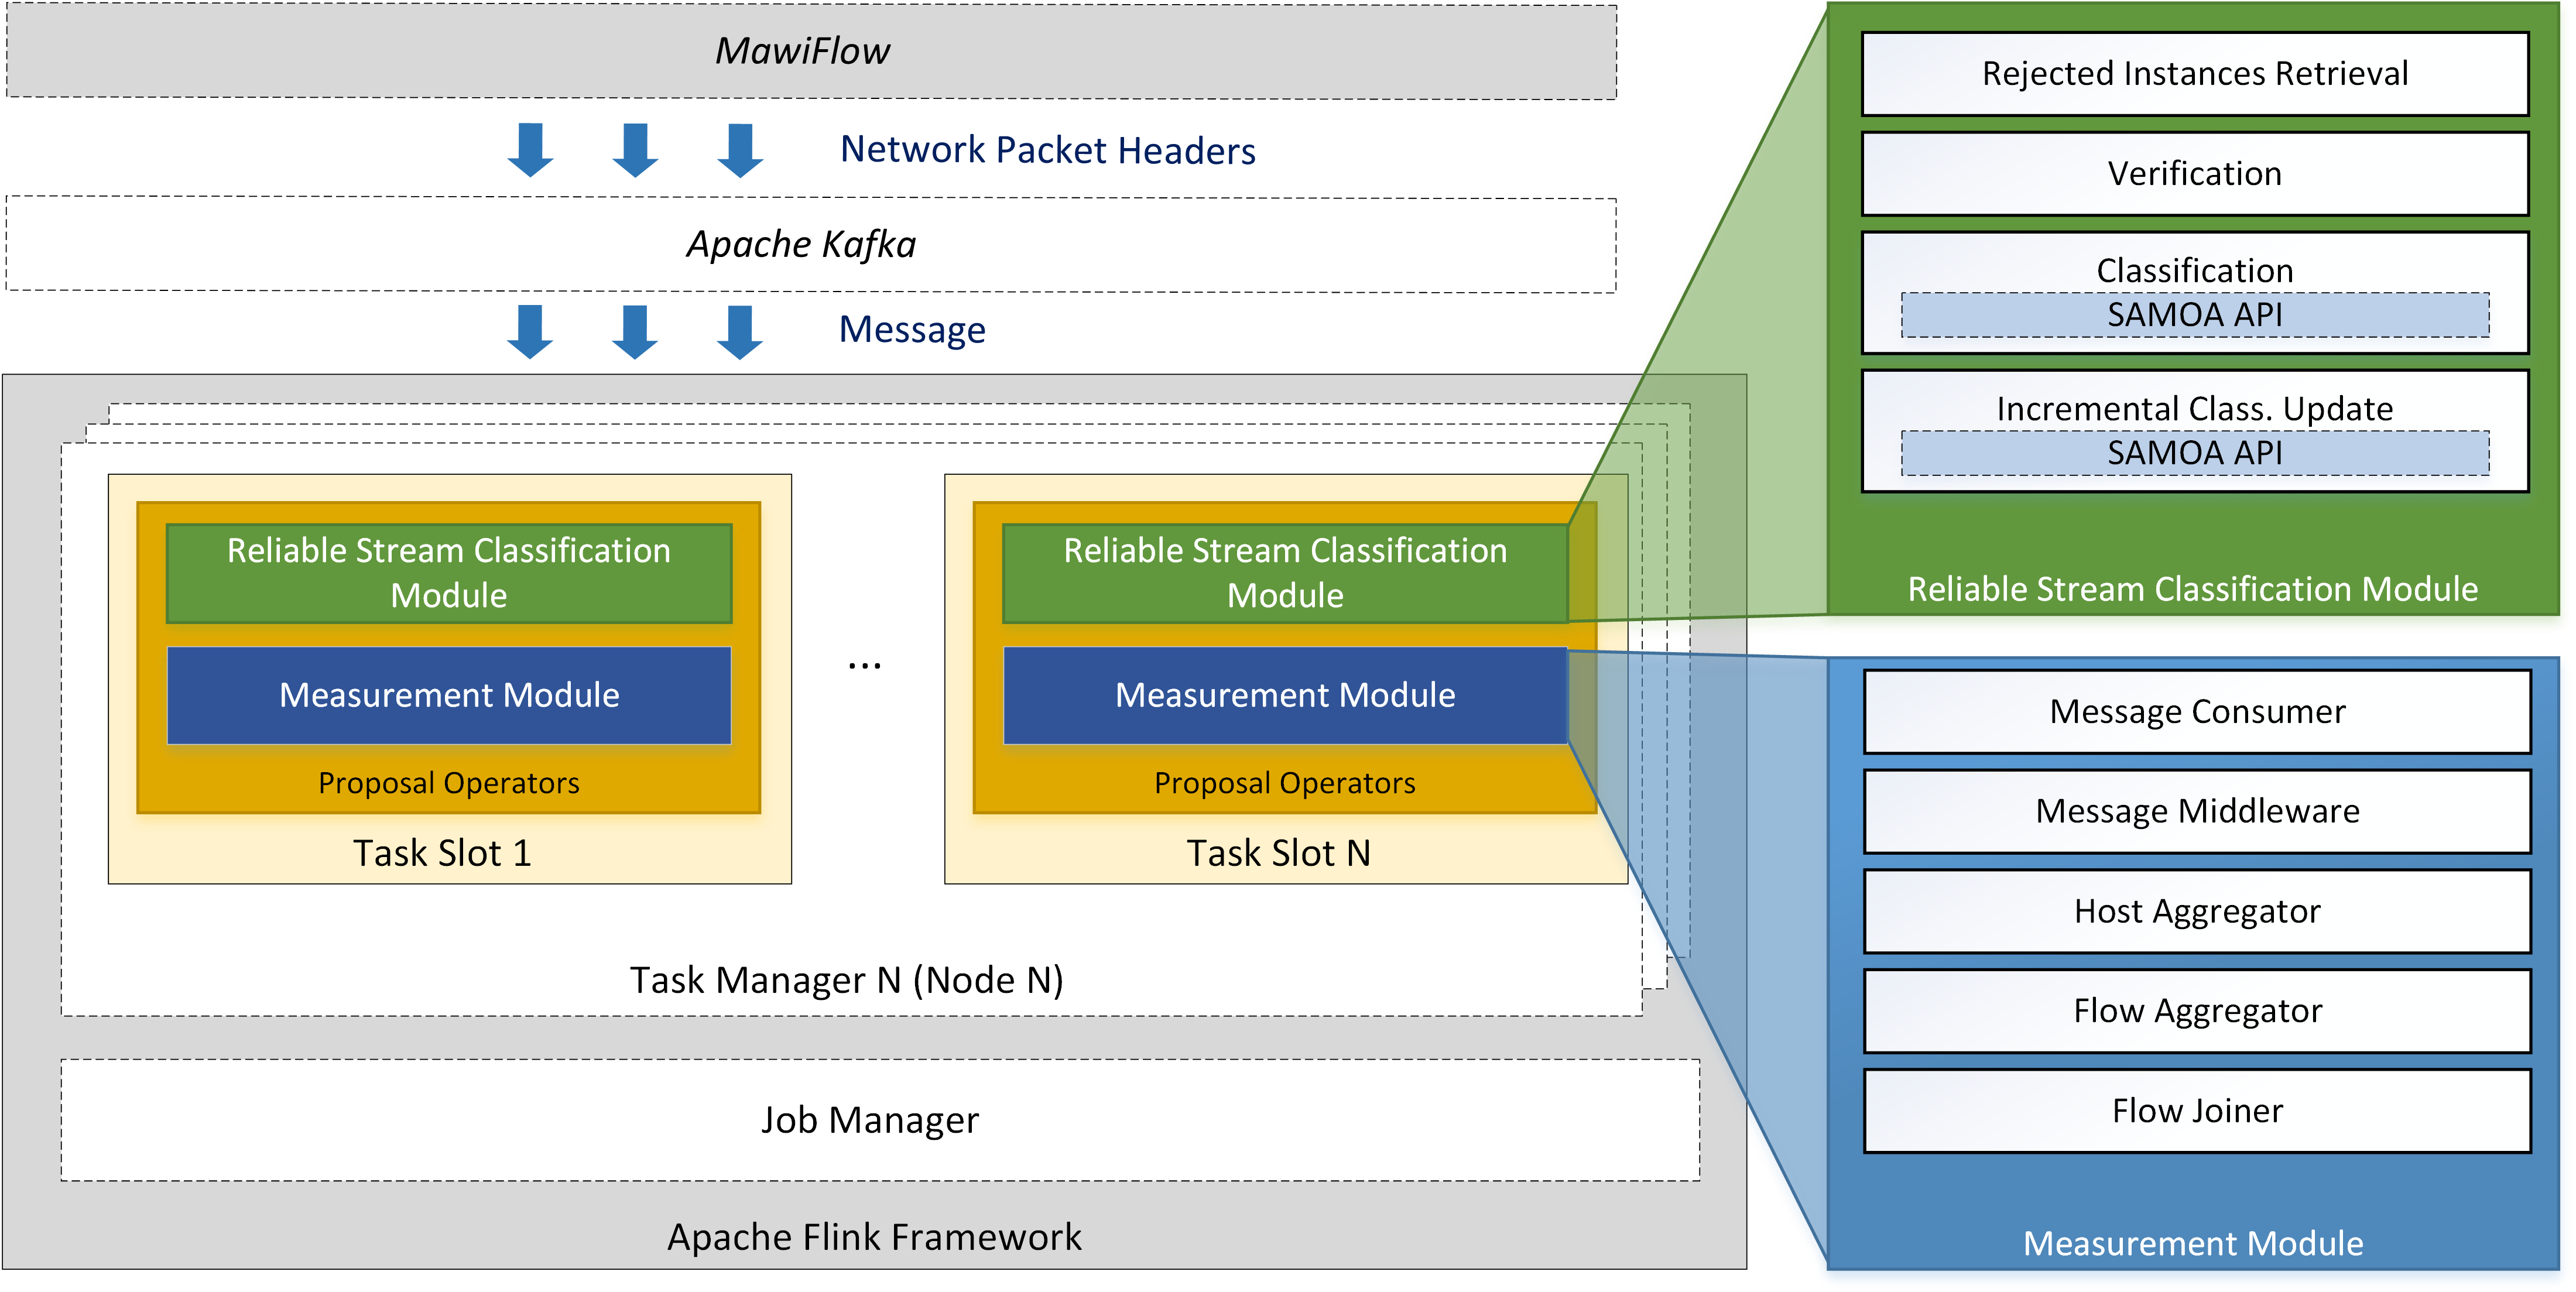
\includegraphics[width=\textwidth]{figuras/bigflow-fig5-bigflow_arch.png}
  \caption{Visão geral da arquitetura e distribuição da ferramenta BigFlow \cite{Viegas2019}.}
  \label{fig:bigflow-arch}
\end{figure}
\nota{BigFlow usa stream mining?\\
- qual é a grande contribuição?\\
- qual é a limitação?}
\end{frame}

\begin{frame}[fragile]{Estado da Arte e Trabalhos Relacionados}
\begin{figure}[ht]
  \centering
  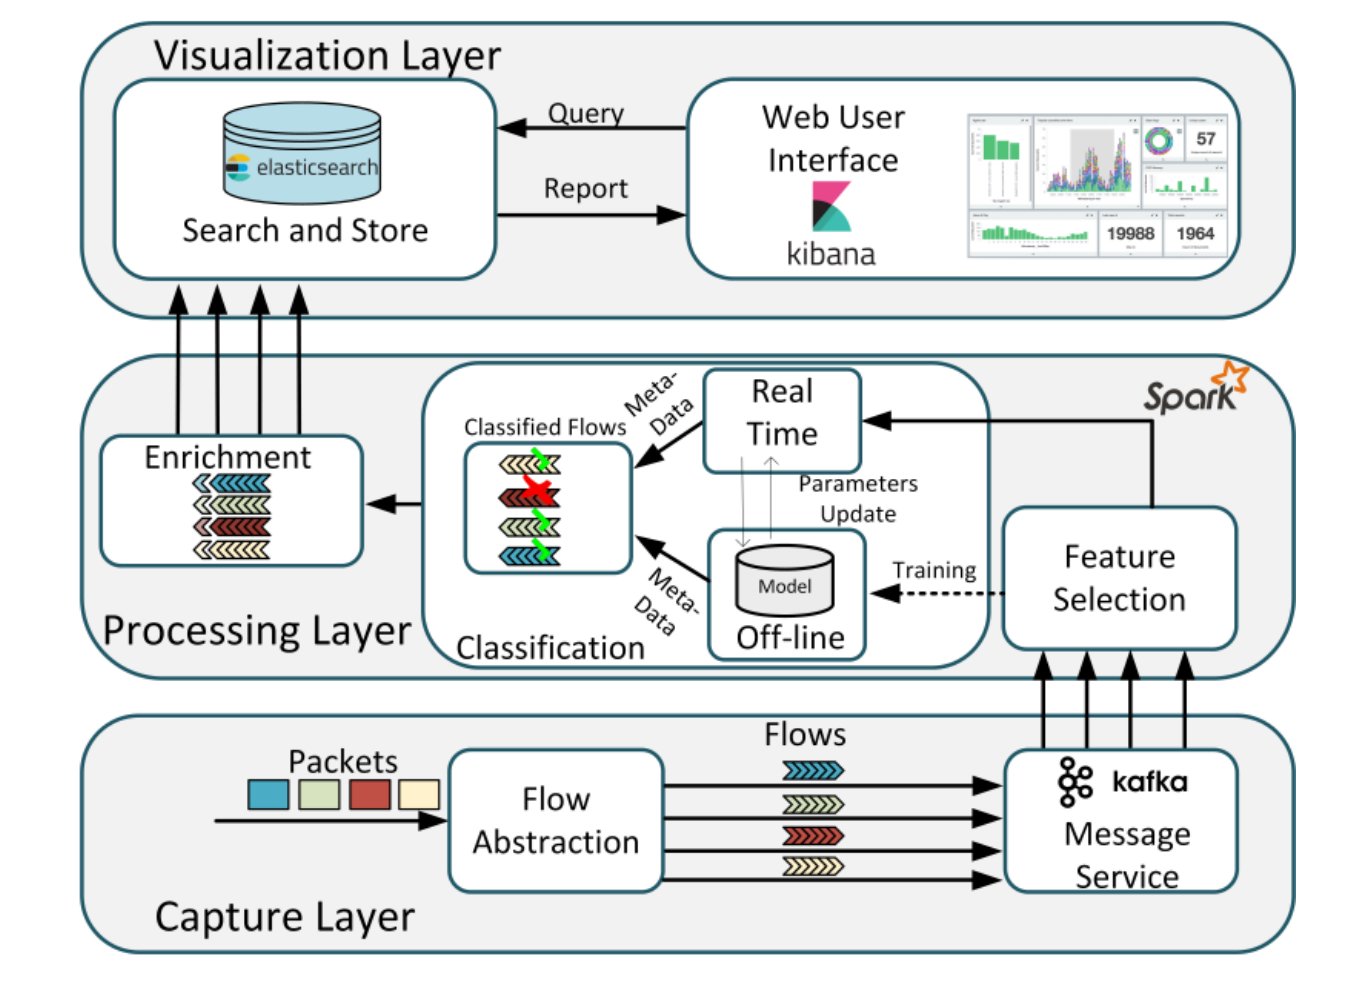
\includegraphics[width=0.8\textwidth]{figuras/catraca-arch.png}
  \caption{Arquitetura em camadas da ferramenta CATRACA \cite{Lopez2018}.}
  \label{fig:catraca}
\end{figure}
\nota{catraca: contribuição? limitação?}
\end{frame}

\begin{frame}[fragile]{Estado da Arte e Trabalhos Relacionados}
\begin{figure}[ht]
  \centering
  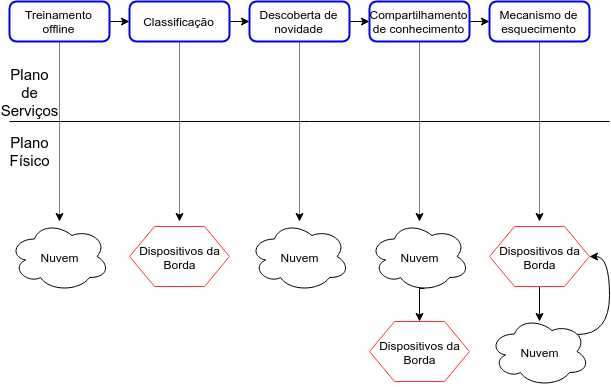
\includegraphics[width=0.8\textwidth]{figuras/idsa-iot-quali-004.png}
  \caption{Distribuição de Serviços da Arquitetura \idsiot.
  Produzida e traduzida por \citeonline{Cassales2019a}.}
  \label{fig:ids-iot}
\end{figure}
\end{frame}

\newcommand{\mfog}{sistema M-FOG\xspace}

\section{Proposta}
\begin{frame}[fragile]{Proposta}
\begin{itemize}
\item Plataforma de processamento distribuído;
\item Arquitetura IDS-IoT;
\item Distribuição do algoritmo MINAS;
\item Validação da implementação por comparação de métricas de qualidade;
\item Métricas de escalabilidade;
\end{itemize}
\nota{Proposta\\
- poderia fazer algumas "perguntas" antes de fazer a sua proposta\\
=> quais perguntas? (voce precisa saber quais)}
\end{frame}


\newcommand{\source}{módulo auxiliar \emph{source}\xspace}
\newcommand{\sink}{módulo auxiliar \emph{sink}\xspace}

\newcommand{\offline}{módulo treinamento\xspace}
\newcommand{\classify}{módulo classificador\xspace}
\newcommand{\detector}{módulo detector de novidades\xspace}

\begin{frame}[fragile]{Proposta}

  O \mfog é dividido em 5 módulos subdivididos em 2 grupos.
  
  \begin{alertblock}{Módulos principais implementam o algoritmo MINAS}
    \begin{itemize}
      \item \offline (\emph{Training Module});
      \item \classify (\emph{Classification Module});
      \item \detector (\emph{Novelty Detection Module}).
    \end{itemize}
  \end{alertblock}
  \begin{alertblock}{Módulos auxiliares, utilizados para avaliação}
    \begin{itemize}
      \item \source (fonte);
      \item \sink (sorvedouro, consumidor final).
    \end{itemize}
  \end{alertblock}
\end{frame}

\begin{frame}[fragile]{Proposta}
\nota{Modulo ou componente?\\
Achei meio confusa a figura, difícil de distinguir:\\
- parte offline vs Online\\
- roda na fog vs roda na nuvem}
\begin{figure}[h]
  \centering
  \includegraphics[width=0.8\textwidth]{figuras/mfog-arch-v2_pt-br.png}
  \caption{Arquitetura e fluxos de dados do \mfog.}
  \label{fig:arch}
\end{figure}
\end{frame}

\section{Resultados Preliminares}
\begin{frame}[fragile]{Resultados Preliminares}

  \begin{alertblock}{Primeira Implementação com \emph{Python} e \emph{Apache Kafka}}
    \begin{itemize}
      \item \emph{Python} é acessível e fornece bibliotecas diversas;
      \item \emph{Apache Kafka} é um sistema de mensagens distribuído;
      \begin{itemize}
        \item Interface de programação com cliente produtor e consumidor;
        \item Mensagens organizadas em tópicos que são distribuídos em partições;
      \end{itemize}
      \item A hipótese de que a carga seria distribuída entre os consumidores,
      uma vez que o consumidor pode selecionar uma partição para leitura;
      \item Em experimento com um produtor, 8 partições e 8 consumidores,
      observou-se que um consumidor processava a maior parte das mensagens,
      poucos consumidores recebiam algumas mensagens e a maioria dos consumidores
      não recebia mensagem alguma.
    \end{itemize}
  \end{alertblock}
\nota{\textsc{cuidado,} o fato de vc não ter conseguido não significa que não é possível\\
concluir que "o sistema não escala ..." (pode citar, só tome cuidado com a conclusão tirada)}
\end{frame}

\begin{frame}[fragile]{Resultados Preliminares}
  \begin{alertblock}{Segunda Implementação com \emph{Apache Flink}}
    \begin{itemize}
      \item Implementação escrita em Scala ou Java;
      \item Processamento de fluxos \emph{Stateful};
      \item Falta de bibliotecas que distribuam algoritmos base como \emph{K-means};
      \item Sistema \emph{M-FOG} em desenvolvimento, atualmente na fase de
      validação através das métricas de qualidade de classificação.
    \end{itemize}
  \end{alertblock}
\nota{métricas: Tem a fórmula? expressão?}

\nota{"Avaliação do fluxo de saída do classificador" isto é uma métrica?}

\nota{Incluir CR}
\end{frame}

\begin{frame}[fragile]{Resultados Preliminares}
  \begin{alertblock}{Métricas e Ambientes}
    \begin{itemize}
      \item Métricas de qualidade de classificação:
      \begin{itemize}
        \item Avaliação do fluxo de saída do classificador;
        \item Uso de uma matriz de confusão ou erro;
        \item Taxa de desconhecidos;
        \item Macro F-score;
      \end{itemize}
      \item Métricas de escalabilidade:
      \begin{itemize}
        \item Número e tipo de processadores;
        \item Uso de memória;
        \item Tempo de processamento;
        \item Taxa de eventos;
        \item Latência entre a produção e classificação.
      \end{itemize}
    \end{itemize}
  \end{alertblock}
\end{frame}

\section{Considerações Finais}
\begin{frame}{Considerações Finais}
Trabalho continua com a finalização da implementação e validação do MFOG com MINAS.
\end{frame}

\begin{frame}{Considerações Finais}

% \begin{enumerate}[label=\Alph*)]
%   \item \label{task:Z} Exame de Qualificação;
%   \item \label{task:A} Desenvolvimento da aplicação;
%   \item \label{task:B} Validação da aplicação em contraste com a implementação
%   MINAS original:
%     \begin{itemize}
%       \item preparação e, se necessário, adaptação da implementação
%       original e \emph{data sets};
%       \item comparação e, se necessário, ajustes à implementação.
%     \end{itemize}
%   \item \label{task:C} Experimentos com \emph{data sets} e estratégias de 
%   distribuição em \emph{fog};
%   \item \label{task:D} Submissão de artigos com resultados de (\ref{task:C}
%   \item \label{task:E} Defesa da Dissertação.
%   % \item \label{task:E} Comparação com outros trabalhos, envolvendo:
%   %   \begin{itemize}
%   %     \item preparação e, se necessário, adaptação dos programas e \emph{data sets};
%   %     \item comparação e publicação dos resultados.
%   %   \end{itemize}
% \end{enumerate}

\noindent\begin{ganttchart}[
  vgrid,
  time slot format=isodate-yearmonth,
  time slot unit=month,
  expand chart=\textwidth,
  inline,
  title height = 1,
  y unit title = 0.6cm,
  y unit chart = 0.7cm,
  bar height = .8,
  bar left shift=.05,
  bar right shift=-.05,
  bar/.style={fill=blue!55, rounded corners=3pt}
]{2020-03}{2020-07}
  \gantttitlecalendar{year, month} \\
  % \ganttmilestone{(\ref{task:Z}}{2020-03-02} \\
  \ganttbar{(Exame de Qualificação)}{2020-03}{2020-03} \\
  \ganttbar{(Desenvolvimento da aplicação)}{2020-03}{2020-03} \\
  \ganttbar{(Validação da aplicação em contraste com a implementaçã)}{2020-03}{2020-04} \\
  \ganttbar{(Experimentos com \emph{data sets} e estratégias de)}{2020-03}{2020-05} \\
  \ganttbar{(Submissão de artigos com resultados de (\ref{task:C)}{2020-04}{2020-07} \\
  \ganttbar{(Defesa da Dissertação)}{2020-06}{2020-07} \\
\end{ganttchart}

\end{frame}

{\setbeamercolor{palette primary}{fg=black, bg=yellow}\begin{frame}[standout]
  Obrigado!
\end{frame}}

\begin{frame}[allowframebreaks]{Referências}
  \bibliography{99.referencias.bib}
\end{frame}

\appendix

\begin{frame}[fragile]{Recomendações de Leitura}
empty
\end{frame}

\end{document}